%%%%%%%%%%%%%%%%%%%%%%%%%%%%%%%%%%%%%%%%%
% KOMA-Script Presentation
% LaTeX Template
% Version 1.0 (3/3/13)
%
% This template has been downloaded from:
% http://www.LaTeXTemplates.com
%
% Original Authors:
% Marius Hofert (marius.hofert@math.ethz.ch)
% Markus Kohm (komascript@gmx.info)
% Described in the PracTeX Journal, 2010, No. 2
%
% License:
% CC BY-NC-SA 3.0 (http://creativecommons.org/licenses/by-nc-sa/3.0/)
%
%%%%%%%%%%%%%%%%%%%%%%%%%%%%%%%%%%%%%%%%%

%----------------------------------------------------------------------------------------
%	PACKAGES AND OTHER DOCUMENT CONFIGURATIONS
%----------------------------------------------------------------------------------------

\documentclass[
paper=128mm:96mm, % The same paper size as used in the beamer class
fontsize=11pt, % Font size
pagesize, % Write page size to dvi or pdf
parskip=half-, % Paragraphs separated by half a line
]{scrartcl} % KOMA script (article)

\linespread{1.12} % Increase line spacing for readability

%------------------------------------------------
% Colors
\usepackage{xcolor}	 % Required for custom colors
% Define a few colors for making text stand out within the presentation
\definecolor{mygreen}{RGB}{44,85,17}
\definecolor{myblue}{RGB}{34,31,217}
\definecolor{mybrown}{RGB}{194,164,113}
\definecolor{myred}{RGB}{255,66,56}
% Use these colors within the presentation by enclosing text in the commands below
\newcommand*{\mygreen}[1]{\textcolor{mygreen}{#1}}
\newcommand*{\myblue}[1]{\textcolor{myblue}{#1}}
\newcommand*{\mybrown}[1]{\textcolor{mybrown}{#1}}
\newcommand*{\myred}[1]{\textcolor{myred}{#1}}
%------------------------------------------------

%------------------------------------------------
% Margins
\usepackage[ % Page margins settings
includeheadfoot,
top=3.5mm,
bottom=3.5mm,
left=5.5mm,
right=5.5mm,
headsep=6.5mm,
footskip=8.5mm
]{geometry}
%------------------------------------------------

%------------------------------------------------
% Fonts
\usepackage[T1]{fontenc}	 % For correct hyphenation and T1 encoding
\usepackage{lmodern} % Default font: latin modern font
%\usepackage{fourier} % Alternative font: utopia
%\usepackage{charter} % Alternative font: low-resolution roman font
\renewcommand{\familydefault}{\sfdefault} % Sans serif - this may need to be commented to see the alternative fonts
%------------------------------------------------

%------------------------------------------------
% Various required packages
\usepackage{amsthm} % Required for theorem environments
\usepackage{bm} % Required for bold math symbols (used in the footer of the slides)
\usepackage{graphicx} % Required for including images in figures
\usepackage{tikz} % Required for colored boxes
\usepackage{booktabs} % Required for horizontal rules in tables
\usepackage{multicol} % Required for creating multiple columns in slides
\usepackage{lastpage} % For printing the total number of pages at the bottom of each slide
\usepackage[english]{babel} % Document language - required for customizing section titles
\usepackage{microtype} % Better typography
\usepackage{tocstyle} % Required for customizing the table of contents

\usepackage{listings}
\usepackage{amssymb}
%------------------------------------------------

%------------------------------------------------
% Slide layout configuration
\usepackage{scrpage2} % Required for customization of the header and footer
\pagestyle{scrheadings} % Activates the pagestyle from scrpage2 for custom headers and footers
\clearscrheadfoot % Remove the default header and footer
\setkomafont{pageheadfoot}{\normalfont\color{black}\sffamily} % Font settings for the header and footer

% Sets vertical centering of slide contents with increased space between paragraphs/lists
\makeatletter
\renewcommand*{\@textbottom}{\vskip \z@ \@plus 1fil}
\newcommand*{\@texttop}{\vskip \z@ \@plus .5fil}
\addtolength{\parskip}{\z@\@plus .25fil}
\makeatother

% Remove page numbers and the dots leading to them from the outline slide
\makeatletter
\newtocstyle[noonewithdot]{nodotnopagenumber}{\settocfeature{pagenumberbox}{\@gobble}}
\makeatother
\usetocstyle{nodotnopagenumber}

\AtBeginDocument{\renewcaptionname{english}{\contentsname}{\Large Outline}} % Change the name of the table of contents
%------------------------------------------------

%------------------------------------------------
% Header configuration - if you don't want a header remove this block
\ihead{
\hspace{-2mm}
\begin{tikzpicture}[remember picture,overlay]
\node [xshift=\paperwidth/2,yshift=-\headheight] (mybar) at (current page.north west)[rectangle,fill,inner sep=0pt,minimum width=\paperwidth,minimum height=2\headheight,top color=mygreen!64,bottom color=mygreen]{}; % Colored bar
\node[below of=mybar,yshift=3.3mm,rectangle,shade,inner sep=0pt,minimum width=128mm,minimum height =1.5mm,top color=black!50,bottom color=white]{}; % Shadow under the colored bar
shadow
\end{tikzpicture}
\color{white}\runninghead} % Header text defined by the \runninghead command below and colored white for contrast
%------------------------------------------------

%------------------------------------------------
% Footer configuration
%\newlength{\footheight}
\setlength{\footheight}{8mm} % Height of the footer
\addtokomafont{pagefoot}{\footnotesize} % Small font size for the footnote

\ifoot{% Left side
\hspace{-2mm}
\begin{tikzpicture}[remember picture,overlay]
\node [xshift=\paperwidth/2,yshift=\footheight] at (current page.south west)[rectangle,fill,inner sep=0pt,minimum width=\paperwidth,minimum height=3pt,top color=mygreen,bottom color=mygreen]{}; % Green bar
\end{tikzpicture}
\myauthor\ \raisebox{0.2mm}{$\bm{\vert}$}\ \myuni % Left side text
}

\ofoot[\pagemark/\pageref{LastPage}\hspace{-2mm}]{\pagemark/\pageref{LastPage}\hspace{-2mm}} % Right side
%------------------------------------------------

%------------------------------------------------
% Section spacing - deeper section titles are given less space due to lesser importance
\usepackage{titlesec} % Required for customizing section spacing
\titlespacing{\section}{0mm}{0mm}{0mm} % Lengths are: left, before, after
\titlespacing{\subsection}{0mm}{0mm}{-1mm} % Lengths are: left, before, after
\titlespacing{\subsubsection}{0mm}{0mm}{-2mm} % Lengths are: left, before, after
\setcounter{secnumdepth}{0} % How deep sections are numbered, set to no numbering by default - change to 1 for numbering sections, 2 for numbering sections and subsections, etc
%------------------------------------------------

%------------------------------------------------
% Theorem style
\newtheoremstyle{mythmstyle} % Defines a new theorem style used in this template
{0.5em} % Space above
{0.5em} % Space below
{} % Body font
{} % Indent amount
{\sffamily\bfseries} % Head font
{} % Punctuation after head
{\newline} % Space after head
{\thmname{#1}\ \thmnote{(#3)}} % Head spec
	
\theoremstyle{mythmstyle} % Change the default style of the theorem to the one defined above
\newtheorem{theorem}{Theorem}[section] % Label for theorems
\newtheorem{remark}[theorem]{Remark} % Label for remarks
\newtheorem{algorithm}[theorem]{Algorithm} % Label for algorithms
\makeatletter % Correct qed adjustment
%------------------------------------------------

%------------------------------------------------
% The code for the box which can be used to highlight an element of a slide (such as a theorem)
\newcommand*{\mybox}[2]{ % The box takes two arguments: width and content
\par\noindent
\begin{tikzpicture}[mynodestyle/.style={rectangle,draw=mygreen,thick,inner sep=2mm,text justified,top color=white,bottom color=white,above}]\node[mynodestyle,at={(0.5*#1+2mm+0.4pt,0)}]{ % Box formatting
\begin{minipage}[t]{#1}
#2
\end{minipage}
};
\end{tikzpicture}
\par\vspace{-1.3em}}
%------------------------------------------------

%----------------------------------------------------------------------------------------
%	PRESENTATION INFORMATION
%----------------------------------------------------------------------------------------

\newcommand*{\mytitle}{Use ACL2 to Verify the Correctness of Lowering Operator when $j=l+s$} % Title
\newcommand*{\runninghead}{The Correctness of Lowering Operators} % Running head displayed on almost all slides
\newcommand*{\myauthor}{Xiaohui Chen} % Presenters name(s)
\newcommand*{\mydate}{\today} % Presentation date
\newcommand*{\myuni}{University of Texas at Austin--Department of Computer Science} % University or department


%----------------------------------------------------------------------------------------

\begin{document}

%----------------------------------------------------------------------------------------
%	TITLE SLIDE
%----------------------------------------------------------------------------------------

% Title slide - you may have to tweak a few of the numbers if you wish to make changes to the layout
\thispagestyle{empty} % No slide header and footer
\begin{tikzpicture}[remember picture,overlay] % Background box
\node [xshift=\paperwidth/2,yshift=\paperheight/2] at (current page.south west)[rectangle,fill,inner sep=0pt,minimum width=\paperwidth,minimum height=\paperheight/2,top color=mygreen,bottom color=mygreen]{}; % Change the height of the box, its colors and position on the page here
\end{tikzpicture}
% Text within the box
\begin{flushright}
\vspace{0.6cm}
\color{white}\sffamily
{\bfseries\Large\mytitle\par} % Title
\vspace{0.5cm}
\normalsize
\myauthor\par % Author name
\mydate\par % Date
\vfill
\end{flushright}

\clearpage

%----------------------------------------------------------------------------------------
%	TABLE OF CONTENT
%----------------------------------------------------------------------------------------

\thispagestyle{empty} % No slide header and footer

\small\tableofcontents % Change the font size and print the table of contents - it may be useful to shrink the font size further if the presentation is full of sections
% To exclude sections/subsections from the table of contents, put an asterisk after \(sub)section like so: \section*{Section Name}

\clearpage

%----------------------------------------------------------------------------------------
%	PRESENTATION SLIDES
%----------------------------------------------------------------------------------------

\section{Clebsch-Gordan Coefficient}


\subsection{Ket notation}

$|j,m_j\rangle$, $|l,m_l\rangle$ ,$|s,m_s\rangle$, etc

$j,m_j,l,m_l,...$ are quantum numbers

The Ket notation represents the state when the particle as the corresponding quantum numbers

\clearpage

%------------------------------------------------

\subsection{The coefficient}

$|j, m_j \rangle = \sum\limits_{m_j = m_l+m_s} c_n |l,m_l\rangle |s,m_s \rangle$

Here $c_n$s  are called the Clebsch-Gordan Coefficients

$|c_n|^2 \equiv$ Given the combined state $|j,ml\rangle$ of a particle, we can know that the particle is in $|l,m_l\rangle|s,m_s\rangle$ with probability $|c_n|^2$

Therefore $\sum\limits_{m_j= m_l+m_s} |c_n|^2 =1$

\clearpage
%------------------------------------------------

\begin{figure}

\centering
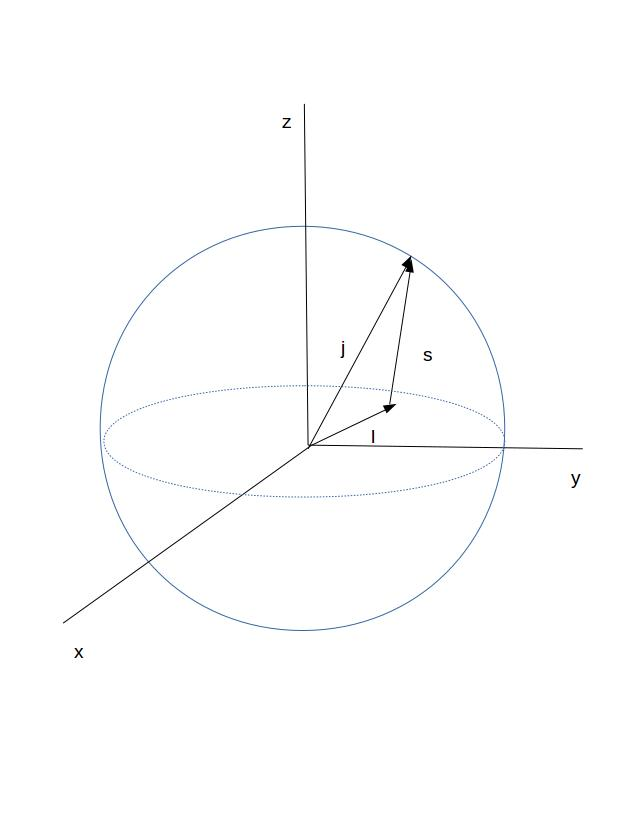
\includegraphics[height=3.2in]{coordinate}

\end{figure}

\clearpage
%------------------------------------------------




\subsection{Lowering-Operators}

\begin{equation}
L_{-} |l\ m_l \rangle = \hbar \sqrt{l(l+1)-m_l(m_l \pm 1)} |l\ (m_l - 1) \rangle
\label{l}
\end{equation}

\begin{equation}
S_{-} |s\ m_s \rangle = \hbar \sqrt{s(s+1)-m_s(m_s - 1)} |s\ (m_s - 1) \rangle
\label{s}
\end{equation}

Since $\vec{j}= \vec{l}+ \vec{s}$, $J_{-}$ obeys the following properties:

\begin{equation}
J_{-}= L_{-} + S_{-}
\label{jsum}
\end{equation}

\begin{equation}
J_{-} |j\ m_j \rangle = \hbar \sqrt{j(j+1)-m_j(m_j - 1)} |s\ (m_j  - 1) \rangle
\label{j}
\end{equation}

\clearpage
%------------------------------------------------

\subsection{Example}

We have an electron with angular momentum $l=1$ and spin $s=\frac{1}{2}$

Therefore $m_l=-1,0,-1$ and $m_s= \pm \frac{1}{2}$

This means $j=\frac{3}{2}$ and $m_j= -\frac{3}{2}, - \frac{1}{2}, \frac{1}{2}, \frac{3}{2}$

We know that the only possibility of forming $|j\ m_j\rangle= |\frac{3}{2}\ \frac{3}{2}\rangle$ is $|\frac{3}{2}\ \frac{3}{2}\rangle = |1\ 1\rangle |\frac{1}{2}\ \frac{1}{2}\rangle $.

Applying the lowering operator on the above equation

$J_{-}|\frac{3}{2}\ \frac{3}{2}\rangle =  \hbar \sqrt{\frac{3}{2} \left( \frac{3}{2}+1 \right) -  \frac{3}{2} \left( \frac{3}{2}-1 \right)} |\frac{3}{2}\ \frac{1}{2}\rangle = \sqrt{3} \hbar |\frac{3}{2}\ \frac{1}{2}\rangle$

$J_{-} |1\ 1\rangle |\frac{1}{2}\ \frac{1}{2}\rangle = (L_{-}+ S_{-}) |1\ 1\rangle |\frac{1}{2}\ \frac{1}{2}\rangle= L_{-}|1\ 1\rangle |\frac{1}{2}\ \frac{1}{2}\rangle + |1\ 1\rangle S_{-} |\frac{1}{2}\ \frac{1}{2}\rangle = \hbar\sqrt{1(1+1)-1(1-1)} |1\ 0\rangle |\frac{1}{2}\ \frac{1}{2}\rangle + \hbar \sqrt{\frac{1}{2} \left( \frac{1}{2}+1 \right) -  \frac{1}{2} \left( \frac{1}{2}-1 \right)} |1\ 1\rangle |\frac{1}{2}\ -\frac{1}{2}\rangle = \hbar \sqrt{2} |1\ 0\rangle |\frac{1}{2}\ \frac{1}{2}\rangle + \hbar |1\ 1\rangle |\frac{1}{2}\ -\frac{1}{2}\rangle$

$\sqrt{3} \hbar |\frac{3}{2}\ \frac{1}{2}\rangle = \hbar \sqrt{2} |1\ 0\rangle |\frac{1}{2}\ \frac{1}{2}\rangle + \hbar |1\ 1\rangle |\frac{1}{2}\ -\frac{1}{2}\rangle$

$\therefore |\frac{3}{2}\ \frac{1}{2}\rangle = \sqrt{\frac{2}{3}} |1\ 0\rangle |\frac{1}{2}\ \frac{1}{2}\rangle + \frac{1}{\sqrt{3}} |1\ 1\rangle |\frac{1}{2}\ -\frac{1}{2}\rangle$


\clearpage
%------------------------------------------------

\section{My Model}

\begin{lstlisting}[language=Lisp,breaklines=true,mathescape]
((A . (j . $m_j$)) .   ;j-state
(B . ((l . $m_l$) . (s . $m_s$))) ;coupled-state
(C . ((l . $m_l$) . (s . $m_s$)))
...)
\end{lstlisting}

or

\begin{lstlisting}[language=Lisp,breaklines=true,mathescape]
(0 . 0) ;This happens when the lowering operators are operated on the lowest states
\end{lstlisting}

\clearpage
%------------------------------------------------


\subsection{Properties of Quantum States}

\begin{enumerate}

\item $A=B+C+ \ldots$

\item $j= |l-s|, |l-s|+1, ... ,l+s$. But here we only consider the case where $j=l+s$

\item $m_j=m_l+m_s$

\item $m_l= -l ,-l+1 ,..., l$, $m_s = -s,-s+1, ... ,s$

\item From the previous condition, we can know that $m_j= -j, -j+1 ,... ,j$

\item $l,s$ can be integers or half-integers (with denominator 2)

\item $m_l, m_s$ can be integers or haldf-integers

\item In my model, j-state and coupled-states are either both 0 or pairs and lists as shown in previous slides

\end{enumerate}
\clearpage
%------------------------------------------------

\section{My Implementation}

\subsection{j-state}

\begin{lstlisting}[language=Lisp,breaklines=true,mathescape]
(A . (j . $m_j$))
\end{lstlisting}

\clearpage
%------------------------------------------------

\subsubsection{Properties}

\begin{lstlisting}[language=Lisp,breaklines=true]
(defun j-coefficient (x) 
	(car x))

(defun quantum-j (x)
	(car (cdr x)))

(defun quantum-mj (x)
	(cdr (cdr x)))

(defun lower-or-lowest-jstate (x)
	 (or (>= (- (quantum-mj x)) (quantum-j x))
	     (equal (j-coefficient x) 0)))

(defun half-or-full-integer (x)
	(xor (equal (denominator x) 1)
	     (equal (denominator x) 2)))

(defun half-full-match (x y)
	(and (iff (equal (denominator x) 1)
		  (equal (denominator y) 1))
	     (iff (equal (denominator x) 2)
		  (equal (denominator y) 2))))

(defun rational-pair (x)
	(if (atom x) 
	    nil
	    (and (rationalp (car x))
		 (< 0 (car x))
		 (rationalp (cdr x))
		 (natp (- (car x) (abs (cdr x))))
		 (half-or-full-integer (car x))
		 (half-or-full-integer (cdr x))
		 (half-full-match (car x) (cdr x))
		 (<= (abs (cdr x)) (car x)))))

(defun true-jstate (a)
	(if (atom a)
	    (equal a 0)
	    (and (rationalp (car a))
		 (<= 0 (car a))
	         (rational-pair (cdr a)))))
\end{lstlisting}

\clearpage
%------------------------------------------------

\subsubsection{J Lowering Operator}

\begin{lstlisting}[language=Lisp,breaklines=true]
(defun j-lowering-operator (x) 
	(if (atom x)
	    0
	    (if (lower-or-lowest-jstate x)
		0
	  	(cons (* (j-coefficient x)
			 (+ (expt (quantum-j x) 2) 
		    	    (quantum-j x)
		            (- (expt (quantum-mj x) 2))
		            (quantum-mj x)))
	              (cons (quantum-j x)
		            (- (quantum-mj x) 1))))))
\end{lstlisting}


\clearpage
%------------------------------------------------

\subsubsection{j-state Theorem}

\begin{lstlisting}[language=Lisp,breaklines=true]
(defthm j-lowering-valid 
	(implies (true-jstate x)
	         (true-jstate (j-lowering-operator x)))
:hints (("Goal" :in-theory 
		(disable same-denominator-add 
			 remove-strict-inequalities 
			 remove-weak-inequalities))))
\end{lstlisting}

\clearpage
%------------------------------------------------

\subsection{Coupled State}

\subsubsection{Properties}

\begin{lstlisting}[language=Lisp,breaklines=true]
(defun first-coupled-state (x)
	(car x))

(defun first-coupled-state-pair (x)
	(cdr (car x)))

(defun first-coupled-coefficient (x)
	(car (first-coupled-state x)))

(defun first-coupled-l-state (x)
	(car (cdr (first-coupled-state x))))
\end{lstlisting}

\begin{lstlisting}[language=Lisp,breaklines=true]
(defun first-coupled-s-state (x)
	(cdr (cdr (first-coupled-state x))))

(defun first-coupled-l (x)
	(car (first-coupled-l-state x)))

(defun first-coupled-ml (x)
	(cdr (first-coupled-l-state x)))

(defun first-coupled-s (x)
	(car (first-coupled-s-state x)))

(defun first-coupled-ms (x)
	(cdr (first-coupled-s-state x)))

\end{lstlisting}

\clearpage
%------------------------------------------------

\begin{lstlisting}[language=Lisp,breaklines=true]
(defun true-coupled-list (x)
	(if (atom x)
	    t
	    (and (rationalp (first-coupled-coefficient x))
		 (<= 0 (first-coupled-coefficient x))
	         (rational-pair (first-coupled-l-state x))
		 (rational-pair (first-coupled-s-state x))
		 (true-coupled-list (cdr x)))))

(defun true-coupled-state (x)
	(if (atom x)
	    (equal x 0)
	    (true-coupled-list x)))
\end{lstlisting}
\clearpage
%------------------------------------------------

\subsubsection{Clean up Zeros in the List}

\begin{lstlisting}[language=Lisp,breaklines=true]
(defun clean-up-zero-list (x) 
	(if (atom x)
	    x
            (if (equal (car x) 0)
		(clean-up-zero-list (cdr x))
	        (cons (car x)
		      (clean-up-zero-list (cdr x))))))
(defun clean-up-zero (x)
	(if (atom x)
	    0
	    (if (all-zeros x)
		0
	        (clean-up-zero-list x))))
\end{lstlisting}

\clearpage
%------------------------------------------------

\subsubsection{clean-up-zero Theorem}

\begin{lstlisting}[language=Lisp,breaklines=true]
(defthm clean-up-zero-valid 
	(implies (true-coupled-state x)
		 (true-coupled-state (clean-up-zero x)))
:hints (("Goal" :in-theory 
		(disable same-denominator-add 
			 remove-strict-inequalities 
			 remove-weak-inequalities))))
\end{lstlisting}
\clearpage
%------------------------------------------------

\subsubsection{l-lowering-operator}

\begin{lstlisting}[language=Lisp,breaklines=true]
(defun l-lowering-operator-helper (x)
	(if (atom x)
	    nil
	    (cons (l-lowering-to-state x) 
		  (l-lowering-operator-helper (cdr x)))))

(defun l-lowering-operator (x)
	(if (atom x)
	    0
	    (clean-up-zero (l-lowering-operator-helper x))))
\end{lstlisting}

\clearpage
%------------------------------------------------

\subsubsection{l-lowering Theorem}

\begin{lstlisting}[language=Lisp,breaklines=true]
(defthm l-lowering-valid 
	(implies (true-coupled-state x)
		 (true-coupled-state (l-lowering-operator x)))
:hints (("Goal" :in-theory 
		(disable same-denominator-add 
			 remove-strict-inequalities 
			 remove-weak-inequalities))))
\end{lstlisting}

\clearpage
%------------------------------------------------

\subsubsection{s-lowering-operator}

\begin{lstlisting}[language=Lisp,breaklines=true]
(defun s-lowering-operator-helper (x)
	(if (atom x)
	    nil
	    (cons (s-lowering-to-state x) 
		  (s-lowering-operator-helper (cdr x)))))

(defun s-lowering-operator (x)
	(if (atom x)
	    0
	    (clean-up-zero (s-lowering-operator-helper x))))
\end{lstlisting}

\clearpage
%------------------------------------------------

\subsubsection{s-lowering Theorem}

\begin{lstlisting}[language=Lisp,breaklines=true]
(defthm s-lowering-valid 
	(implies (true-coupled-state x)
		 (true-coupled-state (s-lowering-operator x)))
:hints (("Goal" :in-theory 
		(disable same-denominator-add 
			 remove-strict-inequalities 
			 remove-weak-inequalities))))
\end{lstlisting}

\clearpage
%------------------------------------------------

\subsection{Merge and Append}

After l-lowering: 

\begin{lstlisting}[language=Lisp,breaklines=true,mathescape]
((A . ((l . $m_l$) . (s . $m_s$))) 
(B . ((l' . $m_l$') . (s' . $m_s$'))))
\end{lstlisting}

After s-lowering:

\begin{lstlisting}[language=Lisp,breaklines=true,mathescape]
((C . ((l' . $m_l$') . (s' . $m_s$'))) 
(D . ((l'' . $m_l$'') . (s'' . $m_s$''))))
\end{lstlisting}

\clearpage
%------------------------------------------------

After append-and-merge-states

\begin{lstlisting}[language=Lisp,breaklines=true,mathescape]
((A . ((l . $m_l$) . (s . $m_s$)))
(E . ((l' . $m_l$') . (s' . $m_s$'))) 
(D . ((l'' . $m_l$'') . (s'' . $m_s$''))))
\end{lstlisting}

$E= [(l+s)^2 - (m_l+m_s)^2 + l+s -m_l -m_s]* \frac{(2l)!(2s)!(l+s+m_l+m_s)!(l+s-m_l- m_s)!}{(2*(l+s))! (l+m_l)!(l-m_l)!(s+m_s)!(s-m_s)!}$\cite{Clebsch}

\clearpage
%------------------------------------------------

\subsubsection{Append and Merge Theorem}

\begin{lstlisting}[language=Lisp,breaklines=true]
(defthm append-valid
        (implies (and (true-coupled-state x)
		      (true-coupled-state y))
	     (true-coupled-state (append-and-merge-states x y))))
\end{lstlisting}

\clearpage
%------------------------------------------------

\subsection{Quantum State}

\begin{lstlisting}[language=Lisp,breaklines=true]
(defun get-jstate (x)
	(car x))

(defun get-coupled-state (x)
	(cdr x))

(defun sum-of-coupled-coefficient (a)
	(if (atom a)
	    0
	    (+ (first-coupled-coefficient a)
	       (sum-of-coupled-coefficient (cdr a)))))
\end{lstlisting}

\clearpage
%------------------------------------------------

\begin{lstlisting}[language=Lisp,breaklines=true]
(defun equal-j (x y)
	(if (atom y)
	    t
	    (and (equal (quantum-j x)
			(+ (first-coupled-l y)
			   (first-coupled-s y)))
		 (equal-j x (cdr y)))))
(defun equal-mj (x y)
	(if (atom y)
	    t
	    (and (equal (quantum-mj x)
			(+ (first-coupled-ml y)
			   (first-coupled-ms y)))
		 (equal-mj x (cdr y)))))
\end{lstlisting}

\clearpage
%------------------------------------------------

\subsubsection{What is a real Quantum state}

\begin{lstlisting}[language=Lisp,breaklines=true]
(defun true-quantum-state (x)
	(xor (and (equal (get-jstate x) 0)
		  (equal (get-coupled-state x) 0))
	     (and (true-jstate (get-jstate x))
		  (true-coupled-state (get-coupled-state x))
		  (equal (sum-of-coupled-coefficient 
				(get-coupled-state x))
			 (caar x))
		  (equal-j (get-jstate x) 
			   (get-coupled-state x))
		  (equal-mj (get-jstate x)
			    (get-coupled-state x)))))
\end{lstlisting}

\clearpage
%------------------------------------------------

\subsection{Normalize}

\begin{lstlisting}[language=Lisp,breaklines=true]
(defun normalize-state (x)
	(if (and (equal (get-jstate x) 0)
		 (equal (get-coupled-state x) 0))
	    x
	    (if (< 0 (car (get-jstate x)))
	        (cons (cons '1 (cdr (get-jstate x)))
		          (normalize-helper (car (get-jstate x)) 
					(get-coupled-state x)))
		(cons '0 '0))))	
\end{lstlisting}


\clearpage
%------------------------------------------------

\subsubsection{Normalize Theorem}

\begin{lstlisting}[language=Lisp,breaklines=true]
(defthm normalize-valid
	(implies (true-quantum-state x)
		 (true-quantum-state (normalize-state x))))
\end{lstlisting}

\clearpage
%------------------------------------------------

\subsection{Quantum Operator}

\begin{lstlisting}[language=Lisp,breaklines=true]
(defun quantum-operator-helper (x)
       (cons (j-lowering-operator (get-jstate x))
	     (append-and-merge-states 
		(l-lowering-operator (get-coupled-state x))
		(s-lowering-operator (get-coupled-state x)))))
(defun quantum-operator (x)
	(if (and (equal (get-jstate x) 0)
		 (equal (get-coupled-state x) 0))
	    x
	(quantum-operator-helper (normalize-state x))))
\end{lstlisting}

\clearpage
%------------------------------------------------


\subsection{Initial State}

\begin{enumerate}

\item ((1 . ($j$ . $m_j$)) . ((1 . (($l$ . $m_l$) . (s . $m_s$)))))

\item $m_l= l$, $m_s=s$, $m_j = j$

\end{enumerate}

For initial state, we can be sure that the coefficients on both sides are 1

\clearpage
%------------------------------------------------

\section{Main Theorem 1}

\begin{lstlisting}[language=Lisp,breaklines=true]
(DEFTHM INITIAL-STATE-LOWERING-VALID
        (IMPLIES (INITIAL-QUANTUM-STATE X)
                 (TRUE-QUANTUM-STATE (QUANTUM-OPERATOR X))))
\end{lstlisting}

\clearpage
%------------------------------------------------

\section{Main Theorem 2 (To be proved in the future)}

\begin{lstlisting}[language=Lisp,breaklines=true]
(skip-proofs
(defun all-lowering-valid (x)
	(if (equal x (cons '0 '0))
	    t
	    (and (true-quantum-state 
			(quantum-operator x))
		 (all-lowering-valid 
			(quantum-operator x)))))

(defthm all-quantum-lowering-valid 
	(implies (inital-quantum-state x)
		 (all-lowering-valid x)))
\end{lstlisting}

\clearpage
%------------------------------------------------

\thispagestyle{empty} % No slide header and footer

\bibliographystyle{unsrt}
\bibliography{sample}

\clearpage
%------------------------------------------------

\thispagestyle{empty} % No slide header and footer

\begin{tikzpicture}[remember picture,overlay] % Background box
\node [xshift=\paperwidth/2,yshift=\paperheight/2] at (current page.south west)[rectangle,fill,inner sep=0pt,minimum width=\paperwidth,minimum height=\paperheight/3,top color=mygreen,bottom color=mygreen]{}; % Change the height of the box, its colors and position on the page here
\end{tikzpicture}
% Text within the box
\begin{flushright}
\vspace{0.6cm}
\color{white}\sffamily
{\bfseries\LARGE Questions?\par} % Request for questions text
\vfill
\end{flushright}

%----------------------------------------------------------------------------------------
\end{document}
